\section{Supplementary materials}\label{sec:SupMat}
\subsection{Experimental support for PSP assumptions}\label{subsec:SupMat1}

The KM-model relies on basic assumptions regarding resource allocation that can
be verified on experimental data collected on isolated individuals of our model
species, the Collembola \textit{Folsomia candida}.

\subsubsection{Methods}

The collembolans are maintained in the laboratory in polyethylene vials
(diameter $52$mm, height $65$mm) filled with a $30$mm width layer of a plaster
of Paris mixed with china ink to facilitate detection of the individuals. Food
is provided by offering small dried pellets of a mixture of agar and dried yeast
in standardized concentration and volume \autocites{tully2008a}.
The rearing boxes where kept in incubators at $21 \pm 0.5\degres$C and the
plaster humidified to maintain a constant humidity within the boxes ($\approx
100\%$ RH). We followed $220$ isolated individuals and regularly measured their
body size (using digital pictures) and fecundity (the size of the layed
clutches).

\subsubsection{Growth trajectories and dependence on resources}

The model supposes that for a constant food level the body length follows a Von
Bertalanffy growth curve, and that the maximum size and the growth rate both
depend on food level. These three aspects are valid for our experimental species
as shown by Figure \ref{Fig4-SM1}.

\begin{figure}[!ht] % Figure 6 
\centering
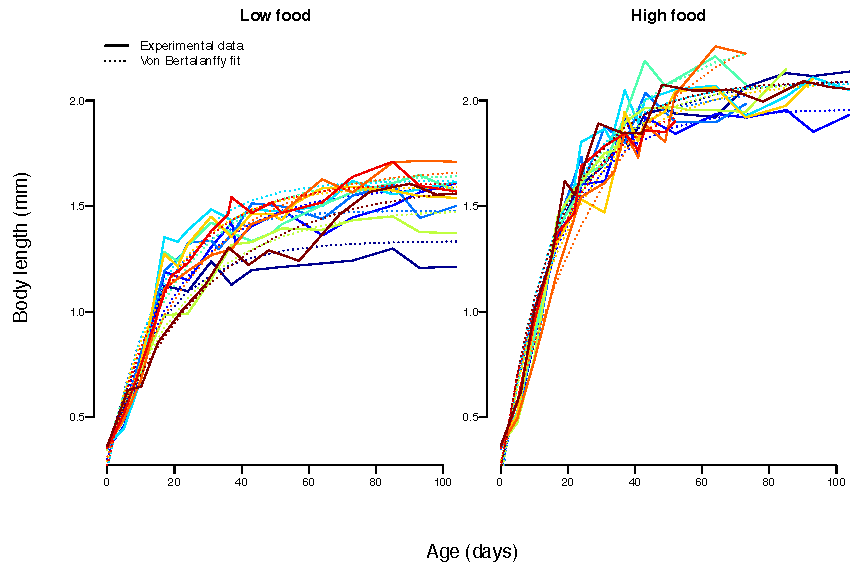
\includegraphics[width=0.85\textwidth]{4_ChapThe1/Fig/FigSM1.pdf} 
\caption[\lofimage{4_ChapThe1/Fig/FigSM1.pdf}Experimental growth
trajectories]{Growth
trajectories (plain lines) and corresponding von Bertalanffy fit  (dotted lines) in two different resource conditions.}
\label{Fig4-SM1}
\end{figure}

\subsubsection{Reproduction}

Furthermore, the KM-model predicts that reproduction increases with the food
level and scales with the square of body length. Figure \ref{Fig4-SM2} shows
that both relations are valid for \textit{F. candida}.

\begin{figure}[!ht] % Figure 6 
\centering
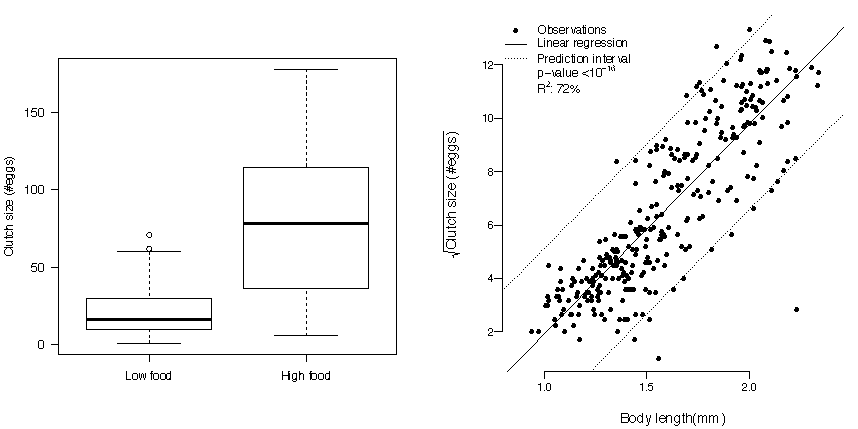
\includegraphics[width=0.85\textwidth]{4_ChapThe1/Fig/FigSM2.pdf}
\caption[\lofimage{4_ChapThe1/Fig/FigSM2.pdf}Experimental measure
of reproduction]{Reproduction (clutch size) in two different resource
conditions, and square root of clutch size against body length. Regression statistics for the latter are extremely significant.}
\label{Fig4-SM2}
\end{figure}

\subsubsection{Size at Birth}

The model assumes that size at birth is independent from food availability.
Figure \ref{Fig4-SM3} shows the egg diameter as a measure correlated to the body
length at birth in two different resource conditions. Although the difference is
significant due to very large sample sizes, the difference between the two means
is quite low and we can consider that the assumption that length at birth is
constant over food availability is valid for our model species.

\begin{figure}[!ht] % Figure 6 
\centering
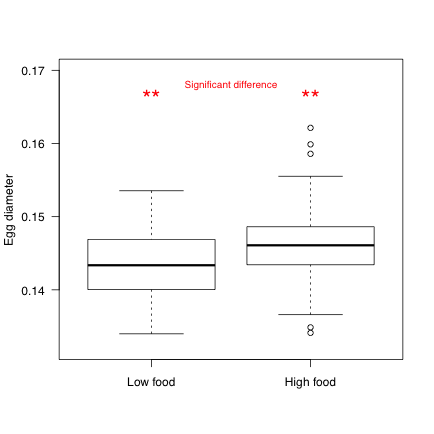
\includegraphics[width=0.7\textwidth]{4_ChapThe1/Fig/FigSM3.pdf}
\caption[\lofimage{4_ChapThe1/Fig/FigSM3.pdf}Experimental measure of size
at birth]{Egg diameter as a proxy for size at birth in two different resource
conditions.}
\label{Fig4-SM3}
\end{figure}

\subsubsection{Maturation length}

Finally, the KM-model assums a length at maturity constant over food
availability and population density. In experimental populations, it is
impossible to assess the body length at maturation. We then realized measures of
size on isolated individuals. This gave us access to the body length at the
first clutch in two different resource conditions, wich is longer than the
length at maturity but the closest proxy available in our experimental
conditions. Figure \ref{Fig4-SM4} shows that the model assumption concerning
length at maturity is not supported by our experimental population. Nevertheless, we
consider that this assumption is not a primary assumption, and considering the
length at maturity constant in the model simplify it without changing
dramatically its behavior.

\begin{figure}[!ht] % Figure 6 
\centering
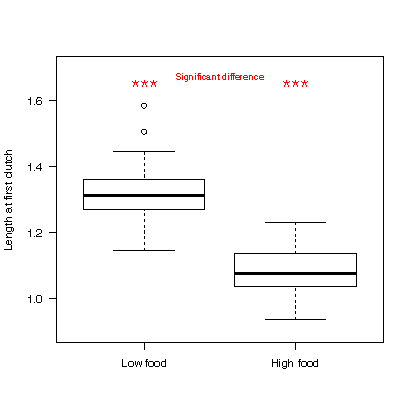
\includegraphics[width=0.7\textwidth]{4_ChapThe1/Fig/FigSM4.pdf}
\caption[\lofimage{4_ChapThe1/Fig/FigSM4.pdf}Experimental measure of
length at maturity]{Length at first clutch in two different resource
conditions.}
\label{Fig4-SM4}
\end{figure}

\subsection{Individual level model}\label{subsec:SupMat2}

Individual interactions being defined as previously described, the individual
rates depend directly on a dynamic energy budget chosen. The choice we made is
based on the $\kappa$-rule \autocite[][Figure
\ref{Fig4-SM5}]{kooijman1984a,de-roos1997a}, which assumes that a fixed
proportion ($\kappa$) of the energy intake (thick black arrow in Figure
\ref{Fig4-SM5}) is allocated to maintenance plus growth while the remainder
($1-\kappa$) goes to reproduction. This implies that when the energy intake goes
down, energy will be rechanneled from growth to maintenance, until growth eventually stops while
reproduction still goes on (dotted arrow in Figure \ref{Fig4-SM5}). For even lower energy
intake, energy will be rechanneled from reproduction to maintenance. This rule
implies that individuals continue reproducing after reaching their maximum size
-- a scenario that is realistic for a wide range of species including
Collembolans. When the energy intake is insufficient to cover maintenance, the
individual is assumed to die.

To be general, let's call $F$ the functionnal response to the resource and $l$
the individual length. In our model, $F$ is the access to the resource
$A(t,l)$.
The energy intake $E_{in}$ of an individual is a function of the functionnal
response and the individual length:
\[ E_{in}=\epsilon\cdot F\cdot l^{2} \]

where $\epsilon$ is a conversion coefficient. And the metabolism
is 
\[
\rho\cdot l^{3}
\]
 where $\rho$ is a parameter. 

\subsubsection*{$\kappa$-rule}\label{subsubsec:SupMat21}


In the $\kappa$-rule, the energy intake (thick black arrow) is first
divided into $1-\kappa$ allocated to reproduction and $\kappa$ allocated
to metabolism, and if all the metabolism cost is paid, the rest of
this $\kappa$ fraction goes to growth (Figure \ref{Fig4-SM5}). 

\begin{figure}[ht] % Figure 6 
\centering
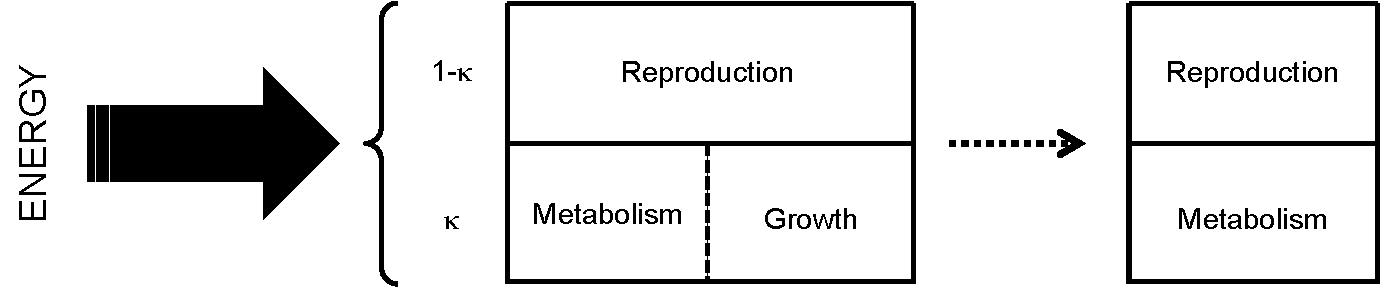
\includegraphics[width=0.95\textwidth]{4_ChapThe1/Fig/KRule}
\caption[\lofimage{4_ChapThe1/Fig/KRule}Details of the
$\kappa$-rule]{Description of the $\kappa$-rule and its implications}
\label{Fig4-SM5}
\end{figure}

Once the individual has reached
it's maximum size (dashed arrow), the energy intake is allocated to
the metabolism and the rest to reproduction. We not that even after
reaching its maximum size, an individual continues to reproduce until
it cannot fulfill its metabolism anymore and dies.

Given the rules of energy allocation, we can write the individual
growth rate and reproduction rate as functions of the functional response
and the individual length.

Birth rate represents the production of newborns (mass or weight $w$)
from the energy absorbed, and can be written:
\begin{eqnarray*}
b_{\kappa}(l) & = & (1-\kappa)\cdot\epsilon\cdot Fl^{2}\\
 & = & r_{m}\cdot Fl^{2}
\end{eqnarray*}


where $r_{m}=(1-\kappa)\cdot\epsilon$ is a reproduction rate. We
note that the birth rate increases with body length following a parabola. 

As opposed to reproduction which is an increase in weight, growth
is the increase in body length $l$. We then define the parameter
$c$ as a length to weight coefficient such as $w=c\cdot l^{3}$,
which leads to 
\[
\frac{dw}{dl}=3c\cdot l^{2}\Leftrightarrow\frac{dl}{dw}=\frac{1}{3cl^{2}}
\]


Expressed in words, growth rate is the fraction $\kappa$ of the energy
intake minus the cost of metabolism. That is to say:

\[
g_{\kappa}(l)=\frac{dl}{dt}=\frac{dw}{dt}\cdot\frac{dl}{dw}=\frac{1}{3cl^{2}}\cdot\frac{dw}{dt}
\]


where $\frac{dw}{dt}$, the change in weight over time is 
\[
\frac{dw}{dt}=\kappa\cdot\epsilon\cdot Fl^{2}-\rho l^{3}
\]
The growth rate in body length is then 
\begin{eqnarray*}
g_{\kappa} & = & \frac{1}{3cl^{2}}\cdot\left(\kappa\cdot\epsilon\cdot Fl^{2}-\rho l^{3}\right)\\
 & = & \frac{1}{3c}\cdot\left(\kappa\cdot\epsilon\cdot F-\rho l\right)\\
 & = & \frac{\rho}{3c}\cdot\left(\frac{\kappa\epsilon}{\rho}F-l\right)
\end{eqnarray*}
Let's define ${\displaystyle \gamma=\frac{\rho}{3c}}$ and ${\displaystyle
l_{m}=\frac{\kappa\epsilon}{\rho}}$, respectively the von Bertalanffy growth
parameter and the absolute maximum length, that is to say the length at infinite resources and
without competition, we can then write the growth rate in the case
of the $\kappa$-rule as follows:

\begin{equation}
g_{\kappa}(l)=\gamma\cdot\left(l_m\cdot F-l\right)
\label{eq:7}
\end{equation}


which integrates as the von Bertalanffy growth function for an isolated
individual. We can see that with the biological interpretations of
$\gamma$ and $l_m$, we don't need to have access to the value
of $\kappa$ to parametrize the model.

\subsubsection{Population level integration}

At the population level, the number of individuals at time t is given by the
integral
\begin{equation}
\label{eq_10}
\int_{l_b}^{l_m}\!n(t,l)\,\mathrm{d}l
\end{equation}
where $n(t,l)$ is the number of individuals of length $l$ at time $t$. The
population dynamics is the described by the following partial differential
equation and limit conditions \autocites{kooijman1984a,de-roos1997a}
\begin{align}
\label{eq_11}
\frac{\partial n(t,l)}{\partial t}+\frac{\partial g(t,l) \cdot n(t,l)}{\partial l}=-\mu \cdot n(t,l) \\
g(t,l_b) \cdot n(t,l_b)= \int_{l_b} ^{l_m} \! b(t,l)\cdot n(t,l)\, \mathrm(d)l
\end{align}
and the initial condition for the population $n(0,l)=\Psi(l)$ where $\Psi(l)$ is
a chosen size distribution. As the $i$-state determines the sate of an
individual, the state of the population, or $p$-state, characterizes the
composition of the structured population modeled, using a density function over
the $i$-states space. 

\newpage
\subsection{Dynamics for I=1.6 and I=1.7}\label{subsec:SupMat3}

\begin{figure}[H] % Figure 6 
\centering
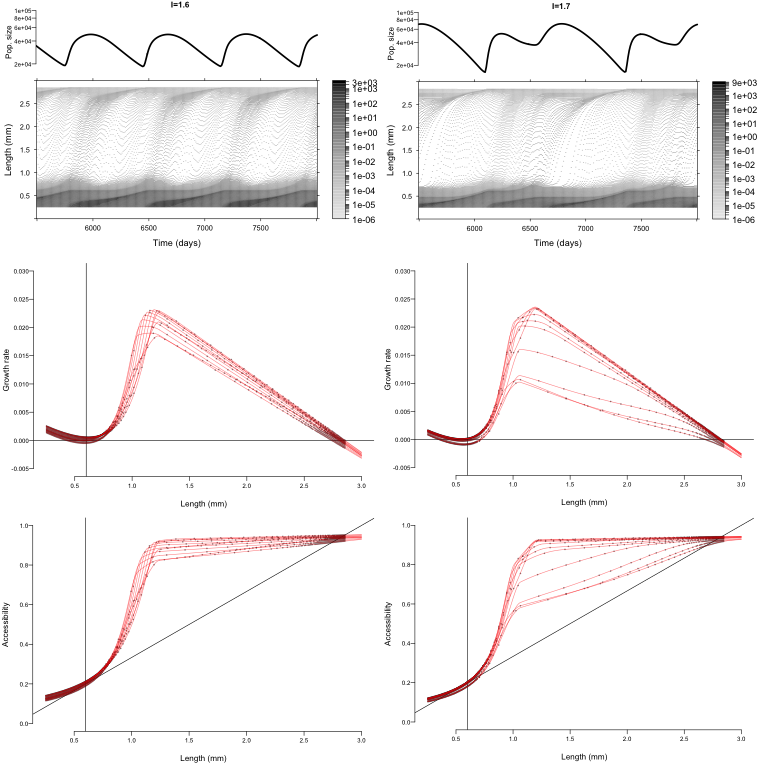
\includegraphics[width=0.95\textwidth]{4_ChapThe1/Fig/FigSM6}
\caption[\lofimage{4_ChapThe1/Fig/FigSM6}Sample dynamics for I=1.6 and
I=1.7]{Population dynamics, growth rate and access to the resource for interference values of $1.6$ and $1.7$. The red lines are the analytical calculations given the state of the population.}
\label{Fig4-SM6}
\end{figure}

\subsection{An alternative energy allocation rule: the net production
model}\label{subsec:SupMat4}

\subsubsection{Description of the Net Production Model}

The $\kappa$-rule is not the only energy allocation rule described in the
literature, although it is one of the most used. Another commonly used rule is the net
production model (Figure \ref{Fig4-SM7}).

\begin{figure}[!ht] % Figure 6 
\centering
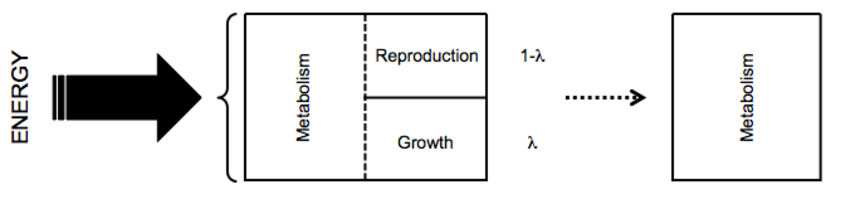
\includegraphics[width=0.95\textwidth]{4_ChapThe1/Fig/FigSM7}
\caption[\lofimage{4_ChapThe1/Fig/FigSM7}Details of the Net
Production model]{Description of the net production model and its implications}
\label{Fig4-SM7}
\end{figure}

In the net production model, the energy intake is first allocated to metabolism.
If some energy is left after fulfilling metabolism, the energy is divided
between growth (fraction $\lambda$) and reproduction (fraction $1-\lambda$).
Once the individual stops growing, meaning it can only fulfill its metabolism, it stops
reproducing at the same time. This is the fundamental difference between the two
rules.

Given the assumptions concerning energy intake and metabolism, we can write the
individual growth rate and reproduction rate as functions of the functional
response and the individual length.

As before, the growth rate in body length can be written as follows:
\[
g_{\text{NP}}=\frac{1}{3cl^{2}}\cdot\frac{dw}{dt}
\]


where $\frac{dw}{dt}$, the change in wheight over time is a fraction
$\lambda$ of what is left after paying for the metabolism: 
\[
\frac{dw}{dt}=\lambda\cdot\left(\epsilon\cdot Fl^{2}-\rho l^{3}\right)
\]


We can hence write the growth rate as follows:
\begin{eqnarray*}
g_{\text{NP}} & = & \frac{1}{3cl^{2}}\cdot\lambda\cdot\left(\epsilon\cdot Fl^{2}-\rho l^{3}\right)\\
 & = & \lambda\cdot\frac{1}{3c}\cdot\left(\epsilon\cdot F-\rho l\right)\\
 & = & \lambda\cdot\frac{\rho}{3c}\cdot\left(\frac{\epsilon}{\rho}F-l\right)
\end{eqnarray*}


Using ${\displaystyle \xi=\lambda\frac{\rho}{3c}}$ and ${\displaystyle L_{NP}=\frac{\epsilon}{\rho}}$
as the von Bertalanffy growth parameter and the absolute maximum length,
we can write the growth rate as:
\[
g_{\text{NP}}(l)=\xi\cdot\left(L_{NP}\cdot F-l\right)
\]


We see that $g_{\kappa}$ and $g_{\text{NP}}$ have the exact same
form. Although the definition of the parameters differ, their biological
interpretation remain the same, with respectively $\gamma$ and $\xi$
the von Bertalanffy growth parameters and $l_m$ and $L_{NP}$ the
absolute maximum length. 

As previously, the birth rate is the increase in mass of newborns:
\[
b_{\text{NP}}(l)=\frac{dw}{dt}\cdot\frac{1}{\omega}
\]
where $\omega$ is the weight of on newborn. With the net production
model, the birth rate is the fraction $1-\lambda$ of the energy left
after fulfilling metabolism:
\begin{eqnarray*}
b_{\text{NP}}(l) & = & \frac{1}{\omega}\cdot(1-\lambda)\cdot\left(\epsilon\cdot Fl^{2}-\rho l^{3}\right)\\
 & = & \frac{1}{\omega}\cdot(1-\lambda)\cdot\rho l^{2}\cdot\left(\frac{\epsilon}{\rho}\cdot F-l\right)
\end{eqnarray*}


Multiplying by $\frac{\lambda}{\lambda}$ we can identify the growth
function $g_{\text{NP}}$:

\begin{eqnarray*}
b_{\text{NP}}(l) & = & \frac{3c}{\omega}\cdot(1-\lambda)\cdot\underbrace{\frac{\lambda}{\lambda}\cdot\frac{\rho}{3c}\cdot\left(\frac{\epsilon}{\rho}\cdot F-l\right)}\cdot l^{2}\\
 & = & \frac{3c}{\omega}\cdot\frac{(1-\lambda)}{\lambda}\cdot\qquad\quad g_{\text{NP}}(l)\;\qquad\cdot l^{2}
\end{eqnarray*}


Furthermore, with $w=3c\cdot l^{3}$, we can write $\omega=c\cdot l_b^{3}$
where $l_b$ is the body length at birth. We then have:
\begin{eqnarray*}
b_{\text{NP}}(l) & = & \frac{(1-\lambda)}{\lambda}\cdot\frac{3}{l_b^{3}}\cdot g_{\text{NP}}(l)\cdot l^{2}
\end{eqnarray*}


We define the parameter ${\displaystyle \beta=\frac{(1-\lambda)}{\lambda}\cdot\frac{3}{l_b^{3}}}$,
and the birth rate writes as
\[
b_{\text{NP}}(l)=\beta\cdot g_{\text{NP}}(l)\cdot l^{2}
\]


We can see that this time that the birth rate is a third degree polynom
which first increases with $l$, and then decreases to $0$ when the
individuals stops growing at $l=l_m\cdot F$.

\subsubsection{From one rule to the other}

In our model, we used the $\kappa$-rule with parameters $\gamma$ and $L_m$
estimated using data from experiments on the collembolan \textit{Folsomia
candida}.
The parameter $L_b$ is also estimated using the same experiments. To convert the
model to a net production energy allocation rule, we can keep the same equation for
the growth function with the same parameters, and simply choose the parameter
$\beta$, knowing the length at birth $L_b$, so that the model behaves similarly
to the $\kappa$-rule model in absence of interference competition and then look at the
effect of interference in the net production model case.

\subsubsection{Bifurcation over interference}

We fixed the value of $\beta$ at $1000$. We then used the same protocol as
described in the methods to investigate the impact of the level of interference on the
dynamics of a structured population in the case of the net production model.

\begin{figure}[!ht] % Figure 6 
\centering
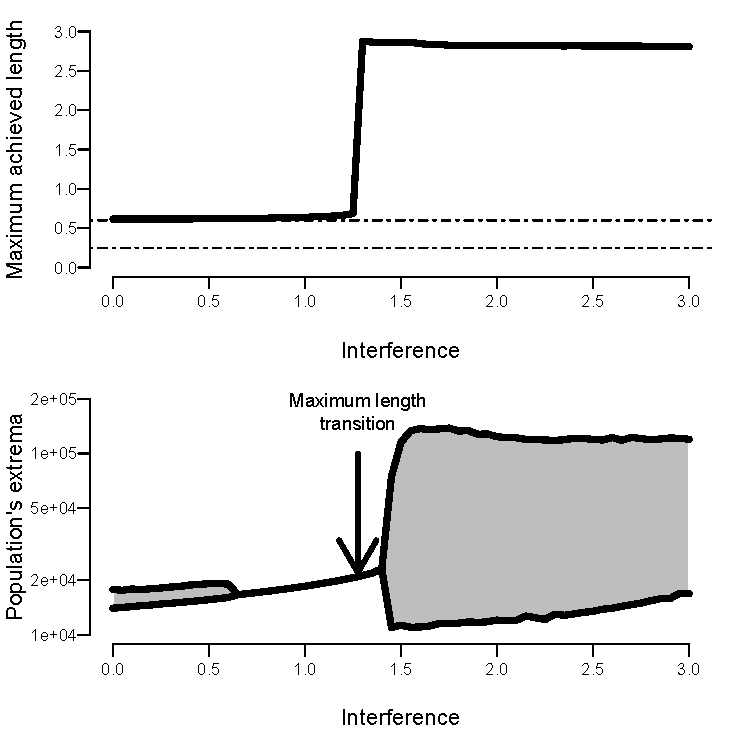
\includegraphics[width=0.95\textwidth]{4_ChapThe1/Fig/FigSM8}
\caption[\lofimage{4_ChapThe1/Fig/FigSM8}Bifurcation over interference
(net production model)]{Maximum achieved length and total population's extremes
for increasing values of interference and a low mortality rate ($\mu=0.0065$).}
\label{Fig4-SM8}
\end{figure}

Figure \ref{Fig4-SM8} shows that the qualitative behavior of the model is the
same as described previously. Indeed, we observe that an increased value of interference
first has a stabilizing effect on the cycles that were present with pure
exploitation.

Furthermore, as previously described, the maximum achieved length in the
population first stays very close to the maturation length but the brutally
reaches a length close to the maximum possible length at infinite resources.
This transition happens in a period where the population structure is stable.

Finally, a higher value of interference destabilizes the structure to limit
cycles with very high amplitude compared to the generation cycles at low
interference. The period of these cycles is also greatly increased, and the
characteristics of the cycles correspond to the “interference-induced cycles”
described for the $\kappa$-rule version of the model.

\subsubsection{Sample simulations}

Looking at sample simulation (Figure \ref{Fig4-SM9} and Figure \ref{Fig4-SM10}),
we can see that although the exact shape of the cycles may differ from the
$\kappa$-rule version, the qualitative dynamics observed for different key
values of interference show the same patterns as previously described. The following figures detail the
population dynamics, the dynamics of the structure, the growth rate as a
function of body length, the access to the resource as a function of body
length, and the birth rate as a function of body length. The birth rate is added
to illustrate the decrease to $0$ when the body growth rate reaches $0$.

\begin{figure}[!ht] % Figure 6 
\centering
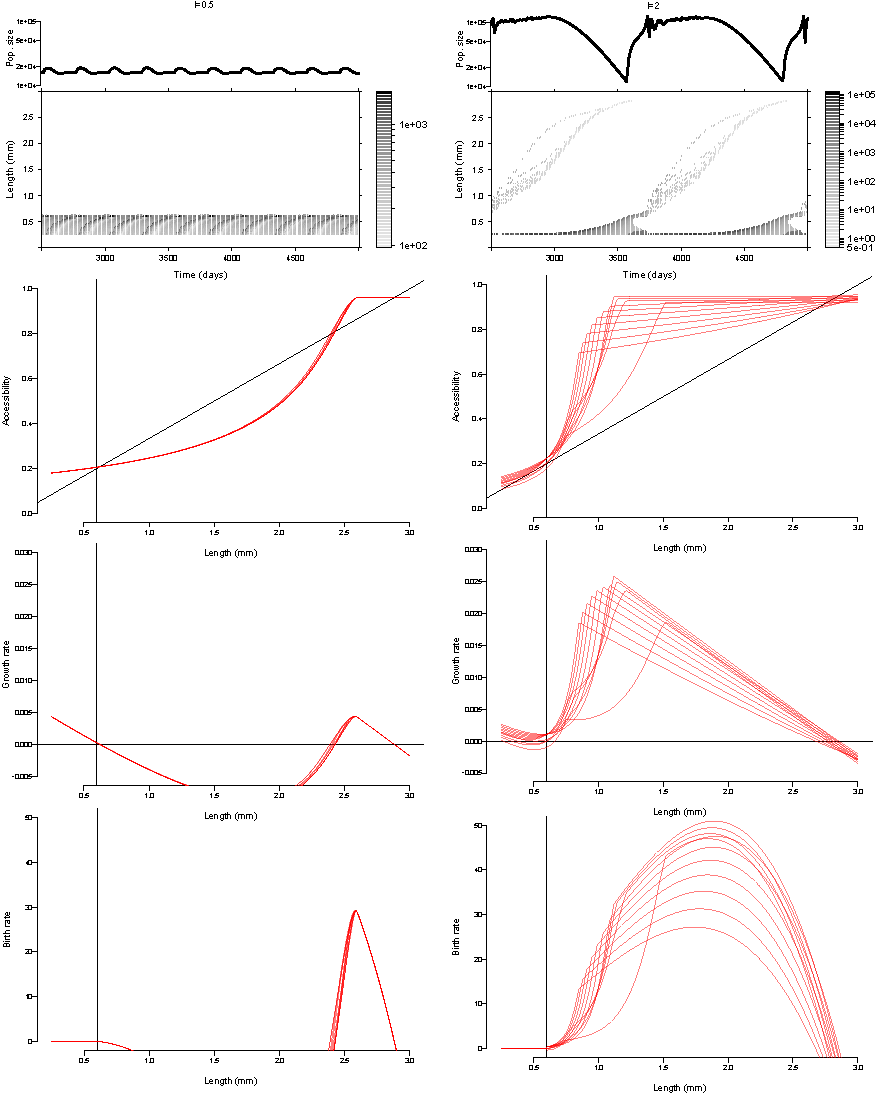
\includegraphics[width=0.95\textwidth]{4_ChapThe1/Fig/FigSM9}
\caption[\lofimage{4_ChapThe1/Fig/FigSM9}Sample simulation for I=0.5
and I=2.0 (net production model)]{Population dynamics, access to the resource,
growth rate and reproduction rate for interference values of $0.5$ and $2.0$. The red lines are the analytical calculations given the state of the population.}
\label{Fig4-SM9}
\end{figure}

\begin{figure}[!ht] % Figure 6 
\centering
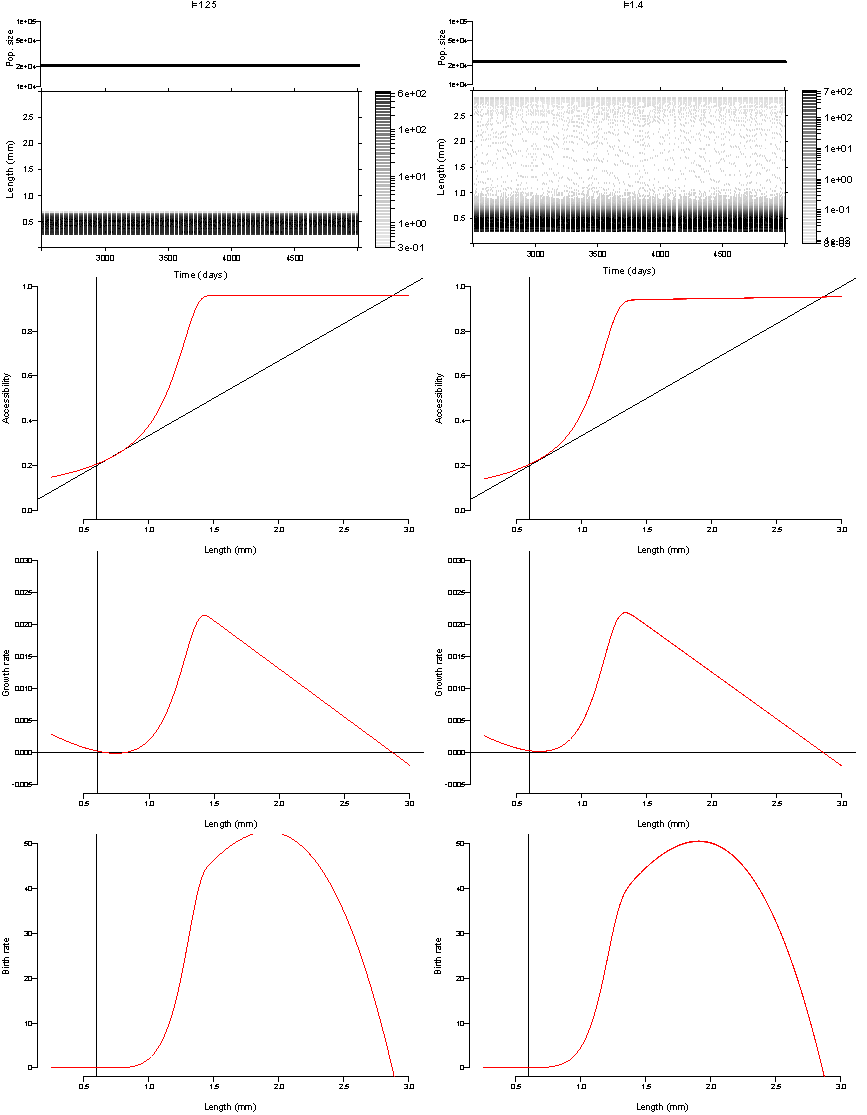
\includegraphics[width=0.95\textwidth]{4_ChapThe1/Fig/FigSM10}
\caption[\lofimage{4_ChapThe1/Fig/FigSM10}Sample simulation for I=1.25
and I=1.45 (net production model)]{Population dynamics, access to the resource,
growth rate and reproduction rate for interference values of $1.25$ and $1.4$. The red lines are
the analytical calculations given the state of the population.}
\label{Fig4-SM10}
\end{figure}

\subsubsection{Discussion}

This study of the model with the net production energy budget implemented showed
that the important results obtained with the $\kappa$-rule version of the model
are still valid under the assumptions of the net production model. This was expected
considering that the dynamics produced by the model with interference are caused
by the progressive superiority acquired by adults while growing when
interference is high. In a population with giant individuals and high
interference, it is the presence of these adults that regulates the population
dynamics rather than the production of young individuals that will compete with
them.

Hence, even though the net production model relies on a very different
assumption concerning reproduction, especially for large individuals, as shown
by Figure \ref{Fig4-SM11} where the birth rate is computed in a case with
infinite resources and no interference, when interference is present, the regulation of
the dynamics shifts from dominated by the juveniles to dominated by the adults,
and the differences between the two energetic rules do not matter in driving the
qualitative dynamics.

\begin{figure}[!ht] % Figure 6 
\centering
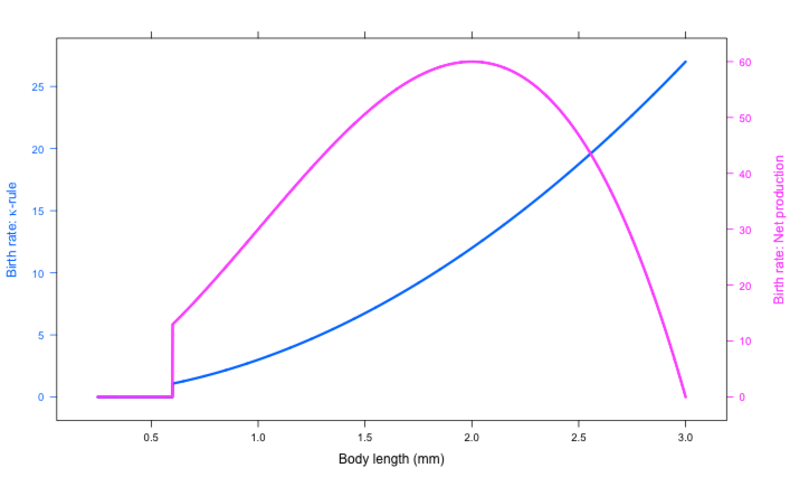
\includegraphics[width=0.95\textwidth]{4_ChapThe1/Fig/FigSM11}
\caption[\lofimage{4_ChapThe1/Fig/FigSM11}Theoretical birth rate for the $\kappa$-rule and the net production model with
$0$ interference]{
Theoretical birth rate for the $\kappa$-rule and the net production model with
$0$ interference.}
\label{Fig4-SM11}
\end{figure}

\subsection{Graphical illustration of competitive superiority of length
\texorpdfstring{$l_{\beta}$}{l_beta} over length
\texorpdfstring{$l_{\alpha}$}{l_alpha}}\label{subsec:SupMat5}

\begin{figure}[!ht] % Figure 6 
\centering
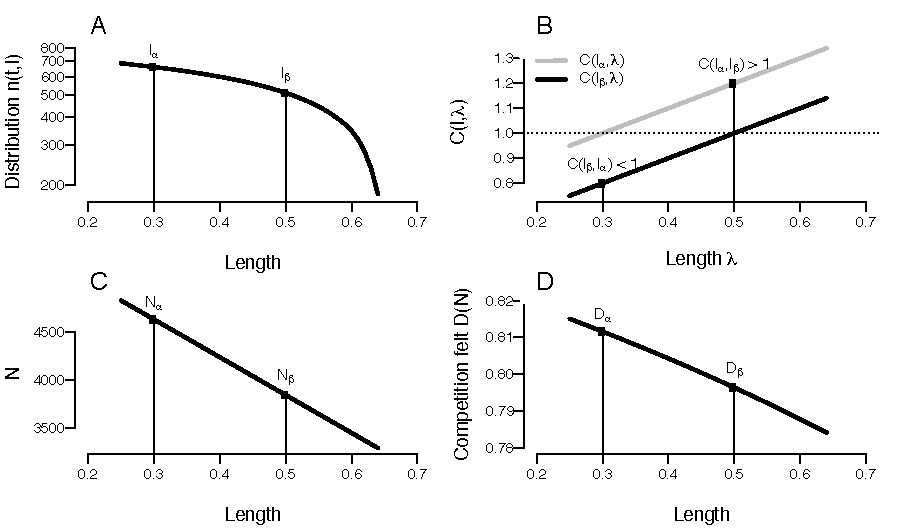
\includegraphics[width=0.95\textwidth]{4_ChapThe1/Fig/FigSM12} 
\caption[\lofimage{4_ChapThe1/Fig/FigSM12}Graphical illustration of competitive superiority of $l_{\beta}$ over
$l_{\alpha}$ when $l_{\alpha}<l_{\beta}$]{
Graphical illustration of competitive superiority of $l_{\beta}$ over
$l_{\alpha}$ when $l_{\alpha}<l_{\beta}$.
(A) Distribution of the size giving the state of the population. (B) Competition
function of individual $\alpha$ (grey) and $\beta$ (black) over every length
present in the population for an interference value of $I=1$. This illustrates
how much individual $\beta$ is competitively superior to individual $\alpha$.
(C) Measure of the environment $\eta(l)$ felt by an individual of length $l$,
given the state of the population in (A). This shows that individual $\alpha$
suffers a denser environment than individual $\beta$. And (D), resource access
for the state of the population given in (A). Individual $\alpha$ suffers a
stronger competition than individual $\beta$.}
\label{Fig4-SM12}
\end{figure}